% Build from docs/: make 2026_10_13_layout_generators.tex
% Figures: docs/images/layout_generators (render.py there regenerates the layouts and schematics);
% the comparator plots come from flow.analysis.runner comp_topology_study / comp_candidate_sweep_study.
% Shared FRIDA Beamer style. Start each slide deck with % Shared FRIDA Beamer style. Start each slide deck with % Shared FRIDA Beamer style. Start each slide deck with \input{style.tex}.
\documentclass[aspectratio=169,compress]{beamer}
\usepackage[T1]{fontenc}
\usepackage{lmodern,graphicx,xcolor,amsmath,booktabs,array,tikz,listings,etoolbox}

% Decks are built from docs/slides; figures live beside docs and in docs/images.
\graphicspath{{../}{./}}

\definecolor{NordBody}{HTML}{4C566A}
\definecolor{NordBlue}{HTML}{5E81AC}
\definecolor{NordRed}{HTML}{BF616A}
\definecolor{NordGreen}{HTML}{A3BE8C}
\definecolor{NordOrange}{HTML}{D08770}
\definecolor{NordPurple}{HTML}{B48EAD}
\definecolor{NordPanel}{HTML}{ECEFF4}

\newcommand{\framesource}{}
\BeforeBeginEnvironment{frame}{\gdef\framesource{}}
\newcommand{\slidesource}[1]{\gdef\framesource{#1}}
\setbeamertemplate{footline}{%
  \hbox{%
    \begin{beamercolorbox}[wd=.12\paperwidth,ht=2.7ex,dp=1.2ex,leftskip=1em]{page number in head/foot}%
      \usebeamerfont{page number in head/foot}\insertframenumber\,/\,\inserttotalframenumber
    \end{beamercolorbox}%
    \begin{beamercolorbox}[wd=.88\paperwidth,ht=2.7ex,dp=1.2ex,right,rightskip=1em]{normal text}%
      \fontsize{5.5}{6.5}\selectfont\ifx\framesource\empty\else Sources:\enspace\framesource\fi
    \end{beamercolorbox}%
  }%
}
\beamertemplatenavigationsymbolsempty
\setbeameroption{hide notes}

% Opt in for decks with sections; shorter decks keep the full frame height.
\newcommand{\slideprogressnavigation}{%
  \useoutertheme[subsection=false]{miniframes}
  \setbeamercolor{section in head/foot}{fg=NordBlue,bg=white}
  \setbeamercolor{mini frame}{fg=NordBlue,bg=white}
  \setbeamercolor{lower separation line head}{bg=NordPanel}
  \setbeamerfont{section in head/foot}{size=\tiny}

  \newif\ifnavbeforecurrent
  \pretocmd\insertnavigation{\navbeforecurrenttrue}{}{}

  \newcommand{\fridanavigationdot}{%
    \begin{pgfpicture}{0pt}{0pt}{0.1cm}{0.1cm}
      \pgfpathcircle{\pgfpoint{0.05cm}{0.05cm}}{0.05cm}
      \ifnavbeforecurrent
        \pgfusepath{fill,stroke}
      \else
        \pgfusepath{stroke}
      \fi
    \end{pgfpicture}%
  }

  \defbeamertemplate*{mini frame}{frida progress}{%
    \begin{pgfpicture}{0pt}{0pt}{0.1cm}{0.1cm}
      \pgfpathcircle{\pgfpoint{0.05cm}{0.05cm}}{0.05cm}
      \pgfusepath{fill,stroke}
    \end{pgfpicture}%
    \global\navbeforecurrentfalse
  }
  \defbeamertemplate*{mini frame in current section}{frida progress}{\fridanavigationdot}
  \defbeamertemplate*{mini frame in current subsection}{frida progress}{\fridanavigationdot}
  \defbeamertemplate*{mini frame in other section}{frida progress}{\fridanavigationdot}
  \defbeamertemplate*{mini frame in other subsection}{frida progress}{\fridanavigationdot}
  \setbeamertemplate{mini frame}[frida progress]
  \setbeamertemplate{mini frame in current section}[frida progress]
  \setbeamertemplate{mini frame in current subsection}[frida progress]
  \setbeamertemplate{mini frame in other section}[frida progress]
  \setbeamertemplate{mini frame in other subsection}[frida progress]
}

\setbeamerfont{frametitle}{size=\large}
\setbeamerfont{framesubtitle}{size=\small}
\setbeamercolor{normal text}{fg=NordBody}
\setbeamercolor{title}{fg=NordBlue}
\setbeamercolor{frametitle}{fg=NordBlue}
\setbeamercolor{framesubtitle}{fg=NordBody}
\setbeamercolor{structure}{fg=NordBlue}
\setbeamercolor{itemize/enumerate body}{fg=NordBody}
\setbeamercolor{itemize/enumerate subbody}{fg=NordBody}
\setbeamercolor{itemize/enumerate subsubbody}{fg=NordBody}
\setbeamercolor{itemize item}{fg=NordBlue}
\setbeamercolor{itemize subitem}{fg=NordBlue}
\setbeamercolor{itemize subsubitem}{fg=NordBlue}
\setbeamercolor{enumerate item}{fg=NordBlue}
\setbeamercolor{enumerate subitem}{fg=NordBlue}
\setbeamercolor{enumerate subsubitem}{fg=NordBlue}
\setbeamercolor{block title}{fg=NordBlue,bg=NordPanel}
\setbeamercolor{block body}{fg=NordBody,bg=NordPanel!55}
\hypersetup{colorlinks=true,allcolors=NordBlue}

\lstset{%
  basicstyle=\ttfamily\tiny,
  keywordstyle=\color{NordBlue}\bfseries,
  commentstyle=\color{NordBody}\itshape,
  stringstyle=\color{NordOrange},
  showstringspaces=false,
  breaklines=true,
  frame=single,
  backgroundcolor=\color{NordPanel!55},
  rulecolor=\color{NordBody!50},
  xleftmargin=2pt,
  xrightmargin=2pt,
  aboveskip=4pt,
  belowskip=4pt,
}

\newcommand{\placeholder}[2]{%
  \begin{tikzpicture}
    \node[minimum width=#1,minimum height=#2,draw=NordBlue!60,rounded corners=2pt,fill=NordPanel,align=center,text=NordBody]
      {Placeholder\\[-1pt]\scriptsize image not yet available};
  \end{tikzpicture}%
}
\newcommand{\maybeimage}[2][]{%
  \IfFileExists{#2}{\includegraphics[#1]{#2}}{%
    \IfFileExists{../#2}{\includegraphics[#1]{#2}}{\placeholder{0.95\linewidth}{0.30\textheight}}%
  }%
}

\author{Kennedy Caisley}
\institute{University of Bonn}
.
\documentclass[aspectratio=169,compress]{beamer}
\usepackage[T1]{fontenc}
\usepackage{lmodern,graphicx,xcolor,amsmath,booktabs,array,tikz,listings,etoolbox}

% Decks are built from docs/slides; figures live beside docs and in docs/images.
\graphicspath{{../}{./}}

\definecolor{NordBody}{HTML}{4C566A}
\definecolor{NordBlue}{HTML}{5E81AC}
\definecolor{NordRed}{HTML}{BF616A}
\definecolor{NordGreen}{HTML}{A3BE8C}
\definecolor{NordOrange}{HTML}{D08770}
\definecolor{NordPurple}{HTML}{B48EAD}
\definecolor{NordPanel}{HTML}{ECEFF4}

\newcommand{\framesource}{}
\BeforeBeginEnvironment{frame}{\gdef\framesource{}}
\newcommand{\slidesource}[1]{\gdef\framesource{#1}}
\setbeamertemplate{footline}{%
  \hbox{%
    \begin{beamercolorbox}[wd=.12\paperwidth,ht=2.7ex,dp=1.2ex,leftskip=1em]{page number in head/foot}%
      \usebeamerfont{page number in head/foot}\insertframenumber\,/\,\inserttotalframenumber
    \end{beamercolorbox}%
    \begin{beamercolorbox}[wd=.88\paperwidth,ht=2.7ex,dp=1.2ex,right,rightskip=1em]{normal text}%
      \fontsize{5.5}{6.5}\selectfont\ifx\framesource\empty\else Sources:\enspace\framesource\fi
    \end{beamercolorbox}%
  }%
}
\beamertemplatenavigationsymbolsempty
\setbeameroption{hide notes}

% Opt in for decks with sections; shorter decks keep the full frame height.
\newcommand{\slideprogressnavigation}{%
  \useoutertheme[subsection=false]{miniframes}
  \setbeamercolor{section in head/foot}{fg=NordBlue,bg=white}
  \setbeamercolor{mini frame}{fg=NordBlue,bg=white}
  \setbeamercolor{lower separation line head}{bg=NordPanel}
  \setbeamerfont{section in head/foot}{size=\tiny}

  \newif\ifnavbeforecurrent
  \pretocmd\insertnavigation{\navbeforecurrenttrue}{}{}

  \newcommand{\fridanavigationdot}{%
    \begin{pgfpicture}{0pt}{0pt}{0.1cm}{0.1cm}
      \pgfpathcircle{\pgfpoint{0.05cm}{0.05cm}}{0.05cm}
      \ifnavbeforecurrent
        \pgfusepath{fill,stroke}
      \else
        \pgfusepath{stroke}
      \fi
    \end{pgfpicture}%
  }

  \defbeamertemplate*{mini frame}{frida progress}{%
    \begin{pgfpicture}{0pt}{0pt}{0.1cm}{0.1cm}
      \pgfpathcircle{\pgfpoint{0.05cm}{0.05cm}}{0.05cm}
      \pgfusepath{fill,stroke}
    \end{pgfpicture}%
    \global\navbeforecurrentfalse
  }
  \defbeamertemplate*{mini frame in current section}{frida progress}{\fridanavigationdot}
  \defbeamertemplate*{mini frame in current subsection}{frida progress}{\fridanavigationdot}
  \defbeamertemplate*{mini frame in other section}{frida progress}{\fridanavigationdot}
  \defbeamertemplate*{mini frame in other subsection}{frida progress}{\fridanavigationdot}
  \setbeamertemplate{mini frame}[frida progress]
  \setbeamertemplate{mini frame in current section}[frida progress]
  \setbeamertemplate{mini frame in current subsection}[frida progress]
  \setbeamertemplate{mini frame in other section}[frida progress]
  \setbeamertemplate{mini frame in other subsection}[frida progress]
}

\setbeamerfont{frametitle}{size=\large}
\setbeamerfont{framesubtitle}{size=\small}
\setbeamercolor{normal text}{fg=NordBody}
\setbeamercolor{title}{fg=NordBlue}
\setbeamercolor{frametitle}{fg=NordBlue}
\setbeamercolor{framesubtitle}{fg=NordBody}
\setbeamercolor{structure}{fg=NordBlue}
\setbeamercolor{itemize/enumerate body}{fg=NordBody}
\setbeamercolor{itemize/enumerate subbody}{fg=NordBody}
\setbeamercolor{itemize/enumerate subsubbody}{fg=NordBody}
\setbeamercolor{itemize item}{fg=NordBlue}
\setbeamercolor{itemize subitem}{fg=NordBlue}
\setbeamercolor{itemize subsubitem}{fg=NordBlue}
\setbeamercolor{enumerate item}{fg=NordBlue}
\setbeamercolor{enumerate subitem}{fg=NordBlue}
\setbeamercolor{enumerate subsubitem}{fg=NordBlue}
\setbeamercolor{block title}{fg=NordBlue,bg=NordPanel}
\setbeamercolor{block body}{fg=NordBody,bg=NordPanel!55}
\hypersetup{colorlinks=true,allcolors=NordBlue}

\lstset{%
  basicstyle=\ttfamily\tiny,
  keywordstyle=\color{NordBlue}\bfseries,
  commentstyle=\color{NordBody}\itshape,
  stringstyle=\color{NordOrange},
  showstringspaces=false,
  breaklines=true,
  frame=single,
  backgroundcolor=\color{NordPanel!55},
  rulecolor=\color{NordBody!50},
  xleftmargin=2pt,
  xrightmargin=2pt,
  aboveskip=4pt,
  belowskip=4pt,
}

\newcommand{\placeholder}[2]{%
  \begin{tikzpicture}
    \node[minimum width=#1,minimum height=#2,draw=NordBlue!60,rounded corners=2pt,fill=NordPanel,align=center,text=NordBody]
      {Placeholder\\[-1pt]\scriptsize image not yet available};
  \end{tikzpicture}%
}
\newcommand{\maybeimage}[2][]{%
  \IfFileExists{#2}{\includegraphics[#1]{#2}}{%
    \IfFileExists{../#2}{\includegraphics[#1]{#2}}{\placeholder{0.95\linewidth}{0.30\textheight}}%
  }%
}

\author{Kennedy Caisley}
\institute{University of Bonn}
.
\documentclass[aspectratio=169,compress]{beamer}
\usepackage[T1]{fontenc}
\usepackage{lmodern,graphicx,xcolor,amsmath,booktabs,array,tikz,listings,etoolbox}

% Decks are built from docs/slides; figures live beside docs and in docs/images.
\graphicspath{{../}{./}}

\definecolor{NordBody}{HTML}{4C566A}
\definecolor{NordBlue}{HTML}{5E81AC}
\definecolor{NordRed}{HTML}{BF616A}
\definecolor{NordGreen}{HTML}{A3BE8C}
\definecolor{NordOrange}{HTML}{D08770}
\definecolor{NordPurple}{HTML}{B48EAD}
\definecolor{NordPanel}{HTML}{ECEFF4}

\newcommand{\framesource}{}
\BeforeBeginEnvironment{frame}{\gdef\framesource{}}
\newcommand{\slidesource}[1]{\gdef\framesource{#1}}
\setbeamertemplate{footline}{%
  \hbox{%
    \begin{beamercolorbox}[wd=.12\paperwidth,ht=2.7ex,dp=1.2ex,leftskip=1em]{page number in head/foot}%
      \usebeamerfont{page number in head/foot}\insertframenumber\,/\,\inserttotalframenumber
    \end{beamercolorbox}%
    \begin{beamercolorbox}[wd=.88\paperwidth,ht=2.7ex,dp=1.2ex,right,rightskip=1em]{normal text}%
      \fontsize{5.5}{6.5}\selectfont\ifx\framesource\empty\else Sources:\enspace\framesource\fi
    \end{beamercolorbox}%
  }%
}
\beamertemplatenavigationsymbolsempty
\setbeameroption{hide notes}

% Opt in for decks with sections; shorter decks keep the full frame height.
\newcommand{\slideprogressnavigation}{%
  \useoutertheme[subsection=false]{miniframes}
  \setbeamercolor{section in head/foot}{fg=NordBlue,bg=white}
  \setbeamercolor{mini frame}{fg=NordBlue,bg=white}
  \setbeamercolor{lower separation line head}{bg=NordPanel}
  \setbeamerfont{section in head/foot}{size=\tiny}

  \newif\ifnavbeforecurrent
  \pretocmd\insertnavigation{\navbeforecurrenttrue}{}{}

  \newcommand{\fridanavigationdot}{%
    \begin{pgfpicture}{0pt}{0pt}{0.1cm}{0.1cm}
      \pgfpathcircle{\pgfpoint{0.05cm}{0.05cm}}{0.05cm}
      \ifnavbeforecurrent
        \pgfusepath{fill,stroke}
      \else
        \pgfusepath{stroke}
      \fi
    \end{pgfpicture}%
  }

  \defbeamertemplate*{mini frame}{frida progress}{%
    \begin{pgfpicture}{0pt}{0pt}{0.1cm}{0.1cm}
      \pgfpathcircle{\pgfpoint{0.05cm}{0.05cm}}{0.05cm}
      \pgfusepath{fill,stroke}
    \end{pgfpicture}%
    \global\navbeforecurrentfalse
  }
  \defbeamertemplate*{mini frame in current section}{frida progress}{\fridanavigationdot}
  \defbeamertemplate*{mini frame in current subsection}{frida progress}{\fridanavigationdot}
  \defbeamertemplate*{mini frame in other section}{frida progress}{\fridanavigationdot}
  \defbeamertemplate*{mini frame in other subsection}{frida progress}{\fridanavigationdot}
  \setbeamertemplate{mini frame}[frida progress]
  \setbeamertemplate{mini frame in current section}[frida progress]
  \setbeamertemplate{mini frame in current subsection}[frida progress]
  \setbeamertemplate{mini frame in other section}[frida progress]
  \setbeamertemplate{mini frame in other subsection}[frida progress]
}

\setbeamerfont{frametitle}{size=\large}
\setbeamerfont{framesubtitle}{size=\small}
\setbeamercolor{normal text}{fg=NordBody}
\setbeamercolor{title}{fg=NordBlue}
\setbeamercolor{frametitle}{fg=NordBlue}
\setbeamercolor{framesubtitle}{fg=NordBody}
\setbeamercolor{structure}{fg=NordBlue}
\setbeamercolor{itemize/enumerate body}{fg=NordBody}
\setbeamercolor{itemize/enumerate subbody}{fg=NordBody}
\setbeamercolor{itemize/enumerate subsubbody}{fg=NordBody}
\setbeamercolor{itemize item}{fg=NordBlue}
\setbeamercolor{itemize subitem}{fg=NordBlue}
\setbeamercolor{itemize subsubitem}{fg=NordBlue}
\setbeamercolor{enumerate item}{fg=NordBlue}
\setbeamercolor{enumerate subitem}{fg=NordBlue}
\setbeamercolor{enumerate subsubitem}{fg=NordBlue}
\setbeamercolor{block title}{fg=NordBlue,bg=NordPanel}
\setbeamercolor{block body}{fg=NordBody,bg=NordPanel!55}
\hypersetup{colorlinks=true,allcolors=NordBlue}

\lstset{%
  basicstyle=\ttfamily\tiny,
  keywordstyle=\color{NordBlue}\bfseries,
  commentstyle=\color{NordBody}\itshape,
  stringstyle=\color{NordOrange},
  showstringspaces=false,
  breaklines=true,
  frame=single,
  backgroundcolor=\color{NordPanel!55},
  rulecolor=\color{NordBody!50},
  xleftmargin=2pt,
  xrightmargin=2pt,
  aboveskip=4pt,
  belowskip=4pt,
}

\newcommand{\placeholder}[2]{%
  \begin{tikzpicture}
    \node[minimum width=#1,minimum height=#2,draw=NordBlue!60,rounded corners=2pt,fill=NordPanel,align=center,text=NordBody]
      {Placeholder\\[-1pt]\scriptsize image not yet available};
  \end{tikzpicture}%
}
\newcommand{\maybeimage}[2][]{%
  \IfFileExists{#2}{\includegraphics[#1]{#2}}{%
    \IfFileExists{../#2}{\includegraphics[#1]{#2}}{\placeholder{0.95\linewidth}{0.30\textheight}}%
  }%
}

\author{Kennedy Caisley}
\institute{University of Bonn}

\slideprogressnavigation

\newcommand{\img}{images/layout_generators}
% the layout renders: build outputs of docs/images/layout_generators/render.py (PDK layouts, never committed)
\newcommand{\lay}{../../build/docs/layout_generators}

% One layout per PDK, scaled by its full cell width (0.065 cm per um) so the six share one scale.
\newcommand{\pdkpanel}[4]{%
  \parbox[b]{#2cm}{\centering\includegraphics[width=#2cm]{\lay/cross_pdk_#1.png}\\[1pt]%
    \makebox[#2cm][c]{\scriptsize #3}\\\makebox[#2cm][c]{\scriptsize #4}}}
\newcommand{\CROSSPDK}{%
  \pdkpanel{tsmc65}{0.941}{TSMC 65}{14.0 $\times$ 10.8 \textmu m}\hspace{12mm}%
  \pdkpanel{ihp130}{2.465}{IHP 130}{37.4 $\times$ 22.7 \textmu m}\hspace{12mm}%
  \pdkpanel{tower180}{2.313}{Tower 180}{34.7 $\times$ 23.5 \textmu m}\par\medskip
  \pdkpanel{tsmc28}{0.785}{TSMC 28}{11.8 $\times$ 5.4 \textmu m}\hspace{12mm}%
  \pdkpanel{lf150}{2.113}{LFoundry 150}{31.0 $\times$ 29.2 \textmu m}\hspace{12mm}%
  \pdkpanel{tpsc65}{1.853}{TPSCo 65}{27.6 $\times$ 14.4 \textmu m}}

% Simulated metrics of the FRIDA-1 baseline and the example (comp_candidate_sweep_study)
\newcommand{\BASENOISE}{0.386}
\newcommand{\BASEPOWER}{4.01}
\newcommand{\BASEENERGY}{160}
\newcommand{\BASESETTLING}{5.51}
\newcommand{\EXNOISE}{0.068}
\newcommand{\EXPOWER}{2.41}
\newcommand{\EXSETTLING}{2.94}
\newcommand{\FREEFRIDA}{20.4 $\times$ 9.0 \textmu m\newline M2+M3 168 \textmu m, 169 vias}
\newcommand{\FREECFORTY}{10.4 $\times$ 10.8 \textmu m\newline 143 \textmu m, 156 vias}
\newcommand{\RINGSTATUS}{Example (shown): 11 decap fingers in 12 row gaps; FRIDA-1: 36 in 10. Both DRC clean and LVS correct}

% TSMC65 wiring of the floorplanned layouts (KLayout extraction, matched to the LVS source on
% every net): area, M2+M3 length, VIA1+VIA2, tail length, latch p/n length mismatch
\newcommand{\wiring}[5]{%
  \par\smallskip
  {\small
  \begin{tabular*}{\linewidth}{@{\extracolsep{\fill}}lccc@{}}
    \toprule
    & cIcCreator & laygo & ALIGN \\
    \midrule
    Area (\textmu m$^2$) & #1 \\
    M2+M3 length (\textmu m) & #2 \\
    VIA1+VIA2 & #3 \\
    Latch p/n length mismatch & #4 \\
    Tail length (\textmu m) & #5 \\
    \bottomrule
  \end{tabular*}
  }}

\title{Comparator layout generators}
\subtitle{From a 297-variant comparator sweep to signoff-clean layouts in three tools and six PDKs}
\date{13 October 2026}

\begin{document}

\begin{frame}
  \titlepage
\end{frame}

\section[Comparator]{Comparator}

\begin{frame}{FRIDA-1 comparator}
  \begin{columns}[c]
    \begin{column}{0.47\textwidth}
      \centering
      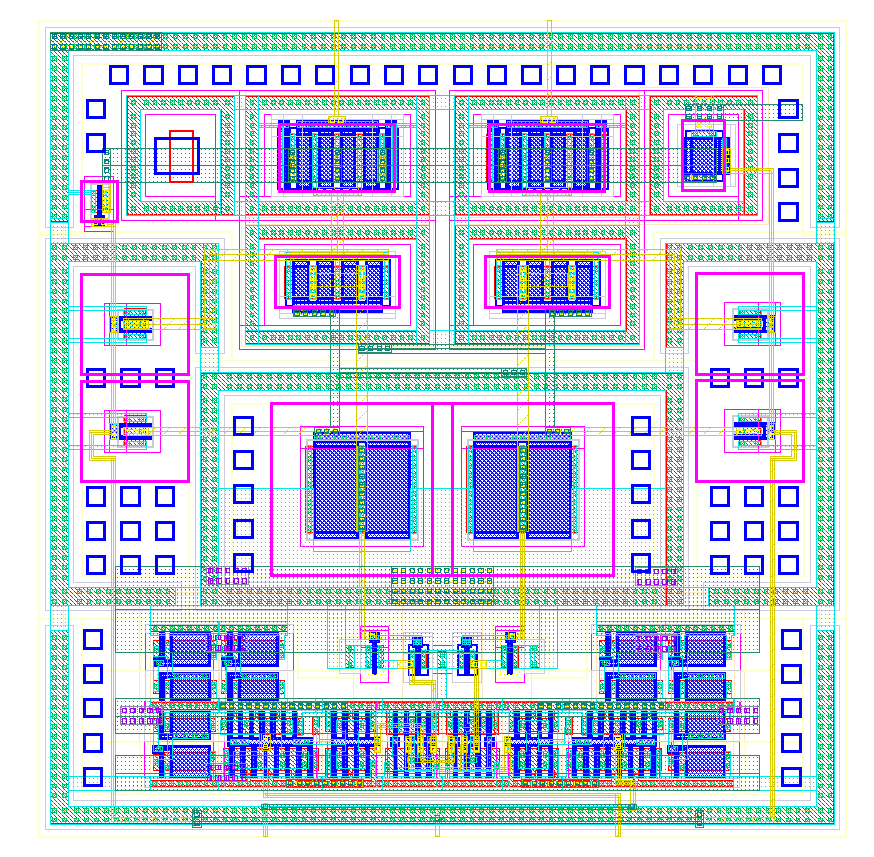
\includegraphics[width=\linewidth,height=0.78\textheight,keepaspectratio]{images/frida_comp.png}
    \end{column}
    \begin{column}{0.5\textwidth}
      \centering
      {\small
      \begin{tabular}{@{}ll@{}}
        \toprule
        Topology & StrongARM, NOR SR latch \\
        Devices & 32 \\
        Layout & 18 $\times$ 18 \textmu m, hand drawn \\
        Input-referred noise & \BASENOISE~mV \\
        Average power & \BASEPOWER~\textmu W \\
        Energy per decision & \BASEENERGY~fJ \\
        Worst settling & \BASESETTLING~ns \\
        \bottomrule
      \end{tabular}
      }
      \par\medskip
      {\scriptsize Schematic simulation of the fabricated dimensions (TSMC65 typical, 1.2 V, 0.8 V common mode, $\pm$3 mV, transient noise), analysed with the current comparator analysis.}
    \end{column}
  \end{columns}
  \slidesource{Sweep baseline \texttt{frida65\_fabricated\_baseline}; \texttt{comp\_candidate\_sweep\_study}}
\end{frame}

\begin{frame}{Six architectures at FRIDA-like sizes}
  \centering
  \includegraphics[width=0.98\linewidth,height=0.74\textheight,keepaspectratio]{\img/comp_topology_study_noise_delay_vs_cm.pdf}
  \par\smallskip
  {\small The four double-tail flavours trade delay against noise differently across common mode; the plain double tail is fastest above 550 mV.}
  \slidesource{\texttt{hdl21\_comp\_topology\_study} (TSMC65, 1.2 V, no mismatch); \texttt{comp\_topology\_study}}
\end{frame}

\begin{frame}{Delay versus input}
  \centering
  \includegraphics[width=0.98\linewidth,height=0.78\textheight,keepaspectratio]{\img/comp_topology_study_delay_vs_input.pdf}
  \slidesource{Median clock-to-decision delay of noise-free decisions, three per point}
\end{frame}

\begin{frame}{297 variants: noise against power}
  \begin{columns}[c]
    \begin{column}{0.68\textwidth}
      \centering
      \maybeimage[width=\linewidth,height=0.8\textheight,keepaspectratio]{\img/comp_candidate_noise_power_tradeoff.pdf}
    \end{column}
    \begin{column}{0.3\textwidth}
      {\small
      \begin{itemize}
        \item 148 topologies at 0.5$\times$ and 2$\times$ FRIDA widths, plus the fabricated baseline
        \item StrongARM and all four double-tail flavours; no triple tail
        \item August simulations (1.2 V, 0.8 V common mode), analysed with the current code
      \end{itemize}
      }
    \end{column}
  \end{columns}
  \slidesource{\texttt{hdl21\_comp\_perf\_vs\_size} (August 2026); \texttt{comp\_candidate\_sweep\_study}}
\end{frame}

\begin{frame}{The example double tail}
  \centering
  \maybeimage[width=0.92\linewidth,height=0.5\textheight,keepaspectratio]{\img/comp_candidate_noise_power_settling.pdf}
  \par\smallskip
  {\small
  \begin{tabular}{@{}lccc@{}}
    \toprule
    & Noise $\sigma$ & Power & Worst settling \\
    \midrule
    FRIDA-1 (StrongARM) & \BASENOISE~mV & \BASEPOWER~\textmu W & \BASESETTLING~ns \\
    Example double tail (c040, 0.5$\times$) & \EXNOISE~mV & \EXPOWER~\textmu W & \EXSETTLING~ns \\
    \bottomrule
  \end{tabular}
  \par\smallskip
  16 of the 200 valid variants reach lower noise, all at higher power; by noise$^2$ $\times$ energy only two (PMOS-input double tails, c120 and c127) do better.
  }
  \slidesource{Double tail with clocked inner-on devices, switched NMOS input}
\end{frame}

\section[Generators]{Generators}

\begin{frame}{Three layout generators}
  \centering
  {\small
  \begin{tabular}{@{}>{\raggedright\arraybackslash}p{0.16\linewidth}*{3}{>{\raggedright\arraybackslash}p{0.26\linewidth}}@{}}
    \toprule
    & cIcCreator & laygo & ALIGN \\
    \midrule
    Input & Object file and SPICE & Python placement script & SPICE and constraints \\
    Placement & Rows, from the floorplan & Rows, from the floorplan & Floorplan, or automatic \\
    Routing & Generator router (M1--M3) & \texttt{route\_net} and track bookkeeping & Automatic (M2--M3) \\
    Runtime & Seconds & Seconds & 20 s to minutes \\
    \bottomrule
  \end{tabular}
  }
  \par\medskip
  {\small
  \begin{itemize}
    \item Tried a year ago without a working flow: each tool needed its own technology description
    \item Now all three draw the same primitives from one description per PDK (\texttt{pdk/<pdk>/layout/tech.py})
    \item Every layout below is Calibre DRC clean and LVS correct (KLayout decks for IHP)
  \end{itemize}
  }
\end{frame}

\begin{frame}{Primitives: transistors}
  \centering
  \includegraphics[width=\linewidth,height=0.42\textheight,keepaspectratio]{\lay/primitives_devices.png}
  \par\medskip
  {\small
  \begin{itemize}
    \item One row cell per device, any $W/L$, fingered to the row: the standard-cell height (1.8 \textmu m, 9 tracks in TSMC65)
    \item Supply rails and well taps under the rails, as in the standard cells
    \item Gate, source and drain reach M2 tracks; the generators route on M2 and M3 only
  \end{itemize}
  }
  \slidesource{TSMC65 row cells of the FRIDA-1 comparator (cIcCreator cell library)}
\end{frame}

\begin{frame}{Primitives: standard cells, row ends and fillers}
  \centering
  \includegraphics[width=\linewidth,height=0.42\textheight,keepaspectratio]{\lay/primitives_cells.png}
  \par\medskip
  {\small
  \begin{itemize}
    \item Library standard cells (decision inverters, SR latch, buffers) sit in the same rows
    \item Each library pin gets an access point on an M2 track, found once per library
    \item Row ends carry the supply stacks; fillers close every gap
  \end{itemize}
  }
  \slidesource{TSMC65 standard-cell library}
\end{frame}

\begin{frame}{Rows: one NMOS, one PMOS}
  \centering
  \includegraphics[width=0.9\linewidth,height=0.62\textheight,keepaspectratio]{\lay/mos_inv_tools.png}
  \par\medskip
  {\small Two rows on a two-row grid (the second flipped, sharing VDD): the same cells in each tool.}
  \slidesource{\texttt{design/layout/mos\_inv.json}}
\end{frame}

\begin{frame}{Schematics, generated from the netlists}
  \centering
  {\small FRIDA-1}\par
  \includegraphics[width=\linewidth,height=0.36\textheight,keepaspectratio]{\img/schematic_comp_frida1.pdf}
  \par\medskip
  {\small Example double tail}\par
  \includegraphics[width=\linewidth,height=0.36\textheight,keepaspectratio]{\img/schematic_comp_c040.pdf}
  \slidesource{\texttt{flow/util/netlist2image.py}: stages in signal-flow order, mirror pairs about each stage's axis}
\end{frame}

\section[Floorplan]{Floorplan}

\begin{frame}[fragile]{Manual floorplan: relative positions only}
  \begin{columns}[c]
    \begin{column}{0.5\textwidth}
\begin{lstlisting}[language={},basicstyle=\ttfamily\tiny]
"rows": [
 ["Mdiff_p", "Mtail", "Mdiff_n"],
 ["Mrst_p", "Mtail_reset", "Mrst_n"],
 ["Mouter_on_p", "Mcross_on_p",
  "Minner_on_p", "Minner_on_n",
  "Mcross_on_n", "Mouter_on_n"],
 ["Minner_init_p", "Mcross_init_p_a",
  "Mcross_init_n_a", "Minner_init_n"],
 ["Mcross_init_n_b", "Mcross_init_p_b"],
 ["Xbuf2_outp", "Xbuf1_outp", "Xsr_p",
  "Xdecision_n", "Xdecision_p", "Xsr_n",
  "Xbuf1_outn", "Xbuf2_outn"]
],
"escape": {"up": ["inp", "inn"],
  "down": ["clk", "clkb", "outp", "outn"]}
\end{lstlisting}
    \end{column}
    \begin{column}{0.47\textwidth}
      {\small
      \begin{itemize}
        \item Rows top first, each left to right, mirrored about the centre
        \item Cross-coupled pairs split into halves for a cross-quad over two rows
        \item Ports escape up or down
        \item One file per design, independent of tool and PDK:
          \begin{itemize}
            \item cIcCreator: row order of its object file
            \item laygo: the placement script
            \item ALIGN: a \texttt{Floorplan} constraint
          \end{itemize}
      \end{itemize}
      }
    \end{column}
  \end{columns}
  \slidesource{\texttt{design/layout/comp\_c040.json}}
\end{frame}

\begin{frame}{FRIDA-1 in three tools}
  \centering
  \includegraphics[width=\linewidth,height=0.5\textheight,keepaspectratio]{\lay/comp_frida1_tools.png}
  \wiring{160 & 160 & 147}{222 & 202 & 164}{212 & 198 & 172}{21\% & 2\% & 1\%}{27.5 & 23.8 & 18.5}
  \slidesource{TSMC65; \texttt{comp\_frida1.json}; length: M2/M3 area over the 100 nm wire width, nets matched to the LVS source}
\end{frame}

\begin{frame}{Example double tail in three tools}
  \centering
  \includegraphics[width=\linewidth,height=0.5\textheight,keepaspectratio]{\lay/comp_c040_tools.png}
  \wiring{151 & 151 & 138}{206 & 198 & 140}{224 & 218 & 159}{5\% & 10\% & 1\%}{17.5 & 14.4 & 10.3}
  \slidesource{TSMC65; \texttt{design/layout/comp\_c040.json}}
\end{frame}

\section[Features]{Features}

\begin{frame}{ALIGN: automatic placement and constraint extraction}
  \begin{columns}[c]
    \begin{column}{0.54\textwidth}
      \centering
      \maybeimage[width=\linewidth,height=0.72\textheight,keepaspectratio]{\lay/align_free.png}
      \par
      {\scriptsize
      \begin{tabular}{@{}>{\centering\arraybackslash}p{0.6\linewidth}>{\centering\arraybackslash}p{0.34\linewidth}@{}}
        FRIDA-1 & Example double tail \\
        \FREEFRIDA & \FREECFORTY \\
      \end{tabular}
      }
    \end{column}
    \begin{column}{0.44\textwidth}
      {\small Input: the netlist and its supplies. Constraints ALIGN extracted for FRIDA-1:}
      \par\smallskip
      {\scriptsize
      \begin{tabular}{@{}ll@{}}
        \toprule
        \texttt{DP\_NMOS} & Mdiff\_p/n \\
        \texttt{CCP\_PMOS} & Mcross\_init\_p/n \\
        \texttt{CCP\_S\_NMOS\_B} & Mcross\_on\_p/n \\
        \texttt{CMC\_PMOS} & Mrst\_p/n \\
        \texttt{CMC\_PMOS} & Minner\_init\_p/n \\
        \midrule
        Symmetric blocks & 7 pairs, 2 groups \\
        Symmetric nets & inp/inn, latch, input drains \\
        & decision, sr, out\_b, out \\
        \bottomrule
      \end{tabular}
      }
      \par\smallskip
      {\small Its symmetry groups merged onto one axis, then placed and routed automatically; DRC clean, LVS correct.}
    \end{column}
  \end{columns}
  \slidesource{\texttt{flow/layout/align/build.py}, no floorplan (TSMC65)}
\end{frame}

\begin{frame}{Cross-PDK compilation: relative sizes, one floorplan}
  \centering
  \CROSSPDK
  \par\smallskip
  {\small Example double tail, to scale (cIcCreator). Sizes in each PDK's unit width and minimum length, so one floorplan fits all six; all 54 layouts DRC clean, LVS correct.}
  \slidesource{\texttt{comp\_c040\_manual\_all\_pdks}; TSMC 65/28, IHP 130, Tower 180, LFoundry 150, TPSCo 65; Calibre (IHP: KLayout)}
\end{frame}

\newcommand{\pdkgallery}[2]{%
\begin{frame}{#2: both designs in three tools}
  \centering
  {\small FRIDA-1}\par
  \includegraphics[width=\linewidth,height=0.34\textheight,keepaspectratio]{\lay/comp_frida1_#1_tools.png}
  \par\medskip
  {\small Example double tail}\par
  \includegraphics[width=\linewidth,height=0.34\textheight,keepaspectratio]{\lay/comp_c040_#1_tools.png}
  \slidesource{\texttt{comp\_frida1\_manual\_all\_pdks}, \texttt{comp\_c040\_manual\_all\_pdks}; one floorplan per design, relative sizes}
\end{frame}}

\pdkgallery{tsmc65}{TSMC 65}
\pdkgallery{ihp130}{IHP 130}
\pdkgallery{tower180}{Tower 180}
\pdkgallery{tsmc28}{TSMC 28}
\pdkgallery{lf150}{LFoundry 150}
\pdkgallery{tpsc65}{TPSCo 65}

\begin{frame}{Guard rings, fill and decap}
  \begin{columns}[c]
    \begin{column}{0.55\textwidth}
      \centering
      \maybeimage[width=\linewidth,height=0.78\textheight,keepaspectratio]{\lay/align_ring.png}
    \end{column}
    \begin{column}{0.43\textwidth}
      {\small
      \begin{itemize}
        \item Row gaps filled with decap cells, their devices added to the LVS source
        \item The block wrapped in the PDK's guard ring (N-well ring on VDD, substrate ring on its own port)
        \item \RINGSTATUS
      \end{itemize}
      }
    \end{column}
  \end{columns}
  \slidesource{decap fill and guard ring (\texttt{PostOptions}); \texttt{flow/layout/align/post.py}}
\end{frame}

\begin{frame}{Summary}
  {\small
  \begin{itemize}
    \item In the 297-variant sweep, the example double tail has 5.7$\times$ less noise than the FRIDA-1 StrongARM at 60\% of its power; no variant beats it on both
    \item cIcCreator, laygo and ALIGN now produce signoff-clean layouts from one primitive library and one floorplan
    \item ALIGN also places without a floorplan, extracting its own symmetry
    \item The same design compiles in six PDKs; guard rings and decap fill finish a block
  \end{itemize}
  }
\end{frame}

\end{document}
